
%%=============================================================================
%% H6 - ZPools & VDEV's
%%=============================================================================

\chapter{Zpools \& VDEV's}
\label{ch:h6}

In dit hoofdstuk worden zpools en diens bouwstenen, VDEV's, wat meer toegelicht. Er wordt ook een demonstratie gegeven over hoe men zpools en VDEV's aanmaakt en wijzigt.

\section{VDEV's: Virtual Devices}

VDEV's (of voluit Virtual Devices) zijn de bouwstenen van storage pools; het zijn een soort van device drivers die elk een bepaalde functionaliteit aanbieden. Er bestaan verschillende soorten VDEV's: zo zijn er bijvoorbeeld striping VDEV's en mirror VDEV's. Ook worden de verschillende RAID-Z-vormen geïmplementeerd met behulp van één of meerdere VDEV's \autocite{ZFSBonwick}.

Conceptueel worden virtual devices voorgesteld in een boomstructuur, waarvan de bladeren de fysieke VDEV's voorstellen; deze VDEV's komen overeen met fysieke apparaten zoals harde schijven. De andere knopen in de boom worden logische VDEV's genoemd omdat ze een groepering vormen van fysieke VDEV's. Zoals in elke boom bestaat er ook in deze structuur van virtual devices een wortel of \textit{root}. De kinderen van deze root VDEV worden de top-level VDEV's genoemd \autocite{Microsystems2006}.

\begin{figure}
  \centering
  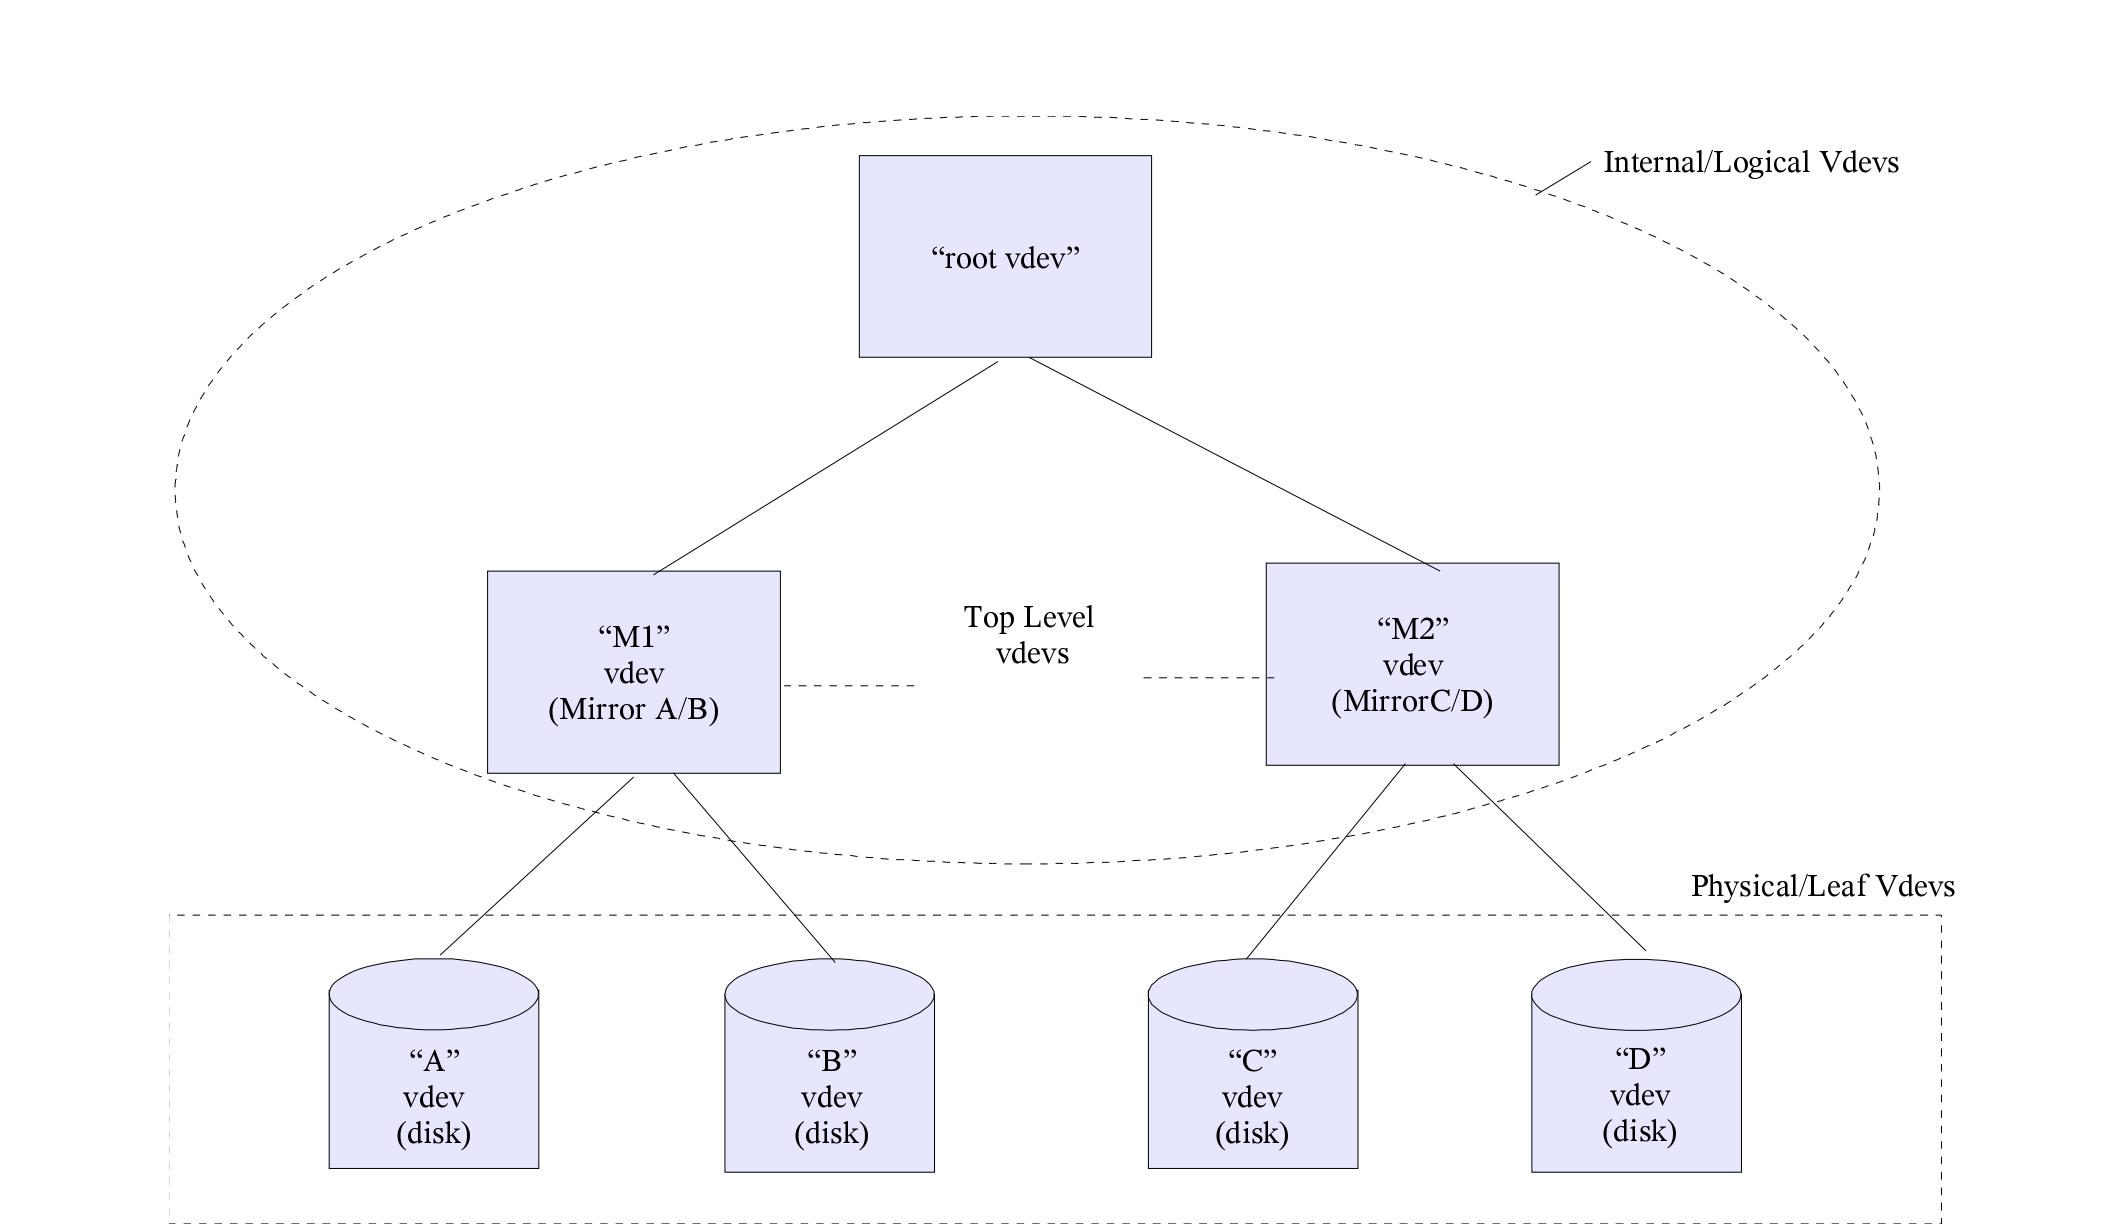
\includegraphics[width=0.9\textwidth]{h6_vdevs_tree}
  \caption{Conceptuele voorstelling van VDEV's in een boomstructuur: M1 en M2 zijn mirrors VDEV's; apparaten A t.e.m. D zijn kinderen van deze VDEV's \autocite{Microsystems2006}.}
  \label{fig:vdevs_boom}
\end{figure}

\lipsum[3-56]
